%%%%%%%%%%%%%%%%%%%%%%%%%%%%%%%%%%%%%%%%%
% Masters/Doctoral Thesis 
% LaTeX Template
% Version 2.5 (27/8/17)
%
% This template was downloaded from:
% http://www.LaTeXTemplates.com
%
% Version 2.x major modifications by:
% Vel (vel@latextemplates.com)
%
% This template is based on a template by:
% Steve Gunn (http://users.ecs.soton.ac.uk/srg/softwaretools/document/templates/)
% Sunil Patel (http://www.sunilpatel.co.uk/thesis-template/)
%
% Template license:
% CC BY-NC-SA 3.0 (http://creativecommons.org/licenses/by-nc-sa/3.0/)
%
%%%%%%%%%%%%%%%%%%%%%%%%%%%%%%%%%%%%%%%%%
%La plantilla base fue utilizada y modificada por Fernando Salazar y Rolando Sotelo
%----------------------------------------------------------------------------------------
%	PACKAGES AND OTHER DOCUMENT CONFIGURATIONS
%----------------------------------------------------------------------------------------

\documentclass[
12pt, % The default document font size, options: 10pt, 11pt, 12pt
%oneside, % Two side (alternating margins) for binding by default, uncomment to switch to one side
english, % ngerman for German
singlespacing, % Single line spacing, alternatives: onehalfspacing or doublespacing
%draft, % Uncomment to enable draft mode (no pictures, no links, overfull hboxes indicated)
%nolistspacing, % If the document is onehalfspacing or doublespacing, uncomment this to set spacing in lists to single
%liststotoc, % Uncomment to add the list of figures/tables/etc to the table of contents
%toctotoc, % Uncomment to add the main table of contents to the table of contents
%parskip, % Uncomment to add space between paragraphs
%nohyperref, % Uncomment to not load the hyperref package
headsepline, % Uncomment to get a line under the header
%chapterinoneline, % Uncomment to place the chapter title next to the number on one line
%consistentlayout, % Uncomment to change the layout of the declaration, abstract and acknowledgements pages to match the default layout
]{MastersDoctoralThesis} % The class file specifying the document structure

\usepackage[utf8]{inputenc} % Required for inputting international characters
\usepackage[T1]{fontenc} % Output font encoding for international characters

\usepackage{mathpazo} % Use the Palatino font by default

\usepackage[backend=biber,style=authoryear,natbib=true]{biblatex} % Use the bibtex backend with the authoryear citation style (which resembles APA)

\addbibresource{example.bib} % The filename of the bibliography

\usepackage[autostyle=true]{csquotes} % Required to generate language-dependent quotes in the bibliography

%----------------------------------------------------------------------------------------
%	MARGIN SETTINGS
%----------------------------------------------------------------------------------------

\geometry{
	paper=a4paper, % Change to letterpaper for US letter
	inner=2.5cm, % Inner margin
	outer=3.8cm, % Outer margin
	bindingoffset=.5cm, % Binding offset
	top=1.5cm, % Top margin
	bottom=1.5cm, % Bottom margin
	%showframe, % Uncomment to show how the type block is set on the page
}

%----------------------------------------------------------------------------------------
%	THESIS INFORMATION
%----------------------------------------------------------------------------------------

\thesistitle{SIMULADOR DE MODELOS DE TRÁFICO PARA NODOS IOT EN UNA RED CELULAR DE 5G} % Your thesis title, this is used in the title and abstract, print it elsewhere with \ttitle
\supervisor{Dr. Domingo \textsc{Lara}} % Your supervisor's name, this is used in the title page, print it elsewhere with \supname
\examiner{} % Your examiner's name, this is not currently used anywhere in the template, print it elsewhere with \examname
\degree{Ingeniería en Telemática} % Your degree name, this is used in the title page and abstract, print it elsewhere with \degreename
\author{Rolando \textsc{Sotelo Alarcón}} % Your name, this is used in the title page and abstract, print it elsewhere with \authorname
\addresses{} % Your address, this is not currently used anywhere in the template, print it elsewhere with \addressname

\subject{Comunicaciones Móviles} % Your subject area, this is not currently used anywhere in the template, print it elsewhere with \subjectname
\keywords{} % Keywords for your thesis, this is not currently used anywhere in the template, print it elsewhere with \keywordnames
\university{\href{http://www.university.com}{Unidad Profesional interdisciplinaria de Ingeniería y Tecnologías Avanzadas}} % Your university's name and URL, this is used in the title page and abstract, print it elsewhere with \univname
\department{\href{http://department.university.com}{Department or School Name}} % Your department's name and URL, this is used in the title page and abstract, print it elsewhere with \deptname
\group{\href{http://researchgroup.university.com}{Research Group Name}} % Your research group's name and URL, this is used in the title page, print it elsewhere with \groupname
\faculty{\href{http://faculty.university.com}{Faculty Name}} % Your faculty's name and URL, this is used in the title page and abstract, print it elsewhere with \facname

\AtBeginDocument{
\hypersetup{pdftitle=\ttitle} % Set the PDF's title to your title
\hypersetup{pdfauthor=\authorname} % Set the PDF's author to your name
\hypersetup{pdfkeywords=\keywordnames} % Set the PDF's keywords to your keywords
}

\begin{document}

\frontmatter % Use roman page numbering style (i, ii, iii, iv...) for the pre-content pages

\pagestyle{plain} % Default to the plain heading style until the thesis style is called for the body content

%----------------------------------------------------------------------------------------
%	TITLE PAGE
%----------------------------------------------------------------------------------------

\begin{titlepage}
\begin{center}

\vspace*{.06\textheight}
{\scshape\LARGE \univname\par}\vspace{1.5cm} % University name
\textsc{\Large Trabajo Terminal}\\[0.5cm] % Thesis type

\HRule \\[0.4cm] % Horizontal line
{\huge \bfseries \ttitle\par}\vspace{0.4cm} % Thesis title
\HRule \\[1.5cm] % Horizontal line
 
\begin{minipage}[t]{0.4\textwidth}
\begin{flushleft} \large
\emph{Author:}\\
\href{http://www.johnsmith.com}{\authorname} % Author name - remove the \href bracket to remove the link
\end{flushleft}
\end{minipage}
\begin{minipage}[t]{0.4\textwidth}
\begin{flushright} \large
\emph{Supervisor:} \\
\href{http://www.jamessmith.com}{\supname} % Supervisor name - remove the \href bracket to remove the link  
\end{flushright}
\end{minipage}\\[3cm]
 
\vfill

\large \textit{A thesis submitted in fulfillment of the requirements\\ for the degree of \degreename}\\[0.3cm] % University requirement text
\textit{in the}\\[0.4cm]
\groupname\\\deptname\\[2cm] % Research group name and department name
 
\vfill

{\large \today}\\[4cm] % Date
%\includegraphics{Logo} % University/department logo - uncomment to place it
 
\vfill
\end{center}
\end{titlepage}

%----------------------------------------------------------------------------------------
%	DECLARATION PAGE
%----------------------------------------------------------------------------------------

\begin{declaration}
\addchaptertocentry{\authorshipname} % Add the declaration to the table of contents
\noindent I, \authorname, declare that this thesis titled, \enquote{\ttitle} and the work presented in it are my own. I confirm that:

\begin{itemize} 
\item This work was done wholly or mainly while in candidature for a research degree at this University.
\item Where any part of this thesis has previously been submitted for a degree or any other qualification at this University or any other institution, this has been clearly stated.
\item Where I have consulted the published work of others, this is always clearly attributed.
\item Where I have quoted from the work of others, the source is always given. With the exception of such quotations, this thesis is entirely my own work.
\item I have acknowledged all main sources of help.
\item Where the thesis is based on work done by myself jointly with others, I have made clear exactly what was done by others and what I have contributed myself.\\
\end{itemize}
 
\noindent Signed:\\
\rule[0.5em]{25em}{0.5pt} % This prints a line for the signature
 
\noindent Date:\\
\rule[0.5em]{25em}{0.5pt} % This prints a line to write the date
\end{declaration}

\cleardoublepage

%----------------------------------------------------------------------------------------
%	QUOTATION PAGE
%----------------------------------------------------------------------------------------

\vspace*{0.2\textheight}

\noindent\enquote{\itshape Thanks to my solid academic training, today I can write hundreds of words on virtually any topic without possessing a shred of information, which is how I got a good job in journalism.}\bigbreak

\hfill Dave Barry

%----------------------------------------------------------------------------------------
%	ABSTRACT PAGE
%----------------------------------------------------------------------------------------

\begin{abstract}
\addchaptertocentry{\abstractname} % Add the abstract to the table of contents
The Thesis Abstract is written here (and usually kept to just this page). The page is kept centered vertically so can expand into the blank space above the title too\ldots
\end{abstract}

%----------------------------------------------------------------------------------------
%	ACKNOWLEDGEMENTS
%----------------------------------------------------------------------------------------

\begin{acknowledgements}
\addchaptertocentry{\acknowledgementname} % Add the acknowledgements to the table of contents
The acknowledgments and the people to thank go here, don't forget to include your project advisor\ldots
\end{acknowledgements}

%----------------------------------------------------------------------------------------
%	LIST OF CONTENTS/FIGURES/TABLES PAGES
%----------------------------------------------------------------------------------------

\tableofcontents % Prints the main table of contents

\listoffigures % Prints the list of figures

\listoftables % Prints the list of tables

%----------------------------------------------------------------------------------------
%	ABBREVIATIONS
%----------------------------------------------------------------------------------------

\begin{abbreviations}{ll} % Include a list of abbreviations (a table of two columns)

\textbf{LAH} & \textbf{L}ist \textbf{A}bbreviations \textbf{H}ere\\
\textbf{WSF} & \textbf{W}hat (it) \textbf{S}tands \textbf{F}or\\

\end{abbreviations}

%----------------------------------------------------------------------------------------
%	PHYSICAL CONSTANTS/OTHER DEFINITIONS
%----------------------------------------------------------------------------------------

\begin{constants}{lr@{${}={}$}l} % The list of physical constants is a three column table

% The \SI{}{} command is provided by the siunitx package, see its documentation for instructions on how to use it

Speed of Light & $c_{0}$ & \SI{2.99792458e8}{\meter\per\second} (exact)\\
%Constant Name & $Symbol$ & $Constant Value$ with units\\

\end{constants}

%----------------------------------------------------------------------------------------
%	SYMBOLS
%----------------------------------------------------------------------------------------

\begin{symbols}{lll} % Include a list of Symbols (a three column table)

$a$ & distance & \si{\meter} \\
$P$ & power & \si{\watt} (\si{\joule\per\second}) \\
%Symbol & Name & Unit \\

\addlinespace % Gap to separate the Roman symbols from the Greek

$\omega$ & angular frequency & \si{\radian} \\

\end{symbols}

%----------------------------------------------------------------------------------------
%	DEDICATION
%----------------------------------------------------------------------------------------

\dedicatory{For/Dedicated to/To my\ldots} 

%----------------------------------------------------------------------------------------
%	Capítulos de la Tesis
%----------------------------------------------------------------------------------------

\mainmatter % Begin numeric (1,2,3...) page numbering

\pagestyle{thesis} % Return the page headers back to the "thesis" style

% Include the chapters of the thesis as separate files from the Chapters folder
% Uncomment the lines as you write the chapters

% Chapter Template

\chapterCapitulo1{Capítulo 1:Presentación del Proyecto} % Main chapter title

\label{Capitulo1} % Change X to a consecutive number; for referencing this chapter elsewhere, use \ref{ChapterX}

%----------------------------------------------------------------------------------------
%	SECTION 1
%----------------------------------------------------------------------------------------

\section{Introducción}



%-----------------------------------
%	SUBSECTION 1
%-----------------------------------
\subsection{Subsection 1}

Nunc posuere quam at lectus tristique eu ultrices augue venenatis. Vestibulum ante ipsum primis in faucibus orci luctus et ultrices posuere cubilia Curae; Aliquam erat volutpat. Vivamus sodales tortor eget quam adipiscing in vulputate ante ullamcorper. Sed eros ante, lacinia et sollicitudin et, aliquam sit amet augue. In hac habitasse platea dictumst.

%-----------------------------------
%	SUBSECTION 2
%-----------------------------------

\subsection{Subsection 2}
Morbi rutrum odio eget arcu adipiscing sodales. Aenean et purus a est pulvinar pellentesque. Cras in elit neque, quis varius elit. Phasellus fringilla, nibh eu tempus venenatis, dolor elit posuere quam, quis adipiscing urna leo nec orci. Sed nec nulla auctor odio aliquet consequat. Ut nec nulla in ante ullamcorper aliquam at sed dolor. Phasellus fermentum magna in augue gravida cursus. Cras sed pretium lorem. Pellentesque eget ornare odio. Proin accumsan, massa viverra cursus pharetra, ipsum nisi lobortis velit, a malesuada dolor lorem eu neque.

%----------------------------------------------------------------------------------------
%	SECTION 2
%----------------------------------------------------------------------------------------

\section{Main Section 2}

Sed ullamcorper quam eu nisl interdum at interdum enim egestas. Aliquam placerat justo sed lectus lobortis ut porta nisl porttitor. Vestibulum mi dolor, lacinia molestie gravida at, tempus vitae ligula. Donec eget quam sapien, in viverra eros. Donec pellentesque justo a massa fringilla non vestibulum metus vestibulum. Vestibulum in orci quis felis tempor lacinia. Vivamus ornare ultrices facilisis. Ut hendrerit volutpat vulputate. Morbi condimentum venenatis augue, id porta ipsum vulputate in. Curabitur luctus tempus justo. Vestibulum risus lectus, adipiscing nec condimentum quis, condimentum nec nisl. Aliquam dictum sagittis velit sed iaculis. Morbi tristique augue sit amet nulla pulvinar id facilisis ligula mollis. Nam elit libero, tincidunt ut aliquam at, molestie in quam. Aenean rhoncus vehicula hendrerit.


\begin{comment}
    \begin{figure}[th]
    \centering
    
\includegraphics{Figures/Electron}
    \decoRule
    \caption[An Electron]{An electron (artist's impression).}
    \label{fig:Electron}
    \end{figure}
\end{comment}



%----------------------------------------------------------------------------------------
%	THESIS CONTENT - APPENDICES
%----------------------------------------------------------------------------------------

\appendix % Cue to tell LaTeX that the following "chapters" are Appendices

% Include the appendices of the thesis as separate files from the Appendices folder
% Uncomment the lines as you write the Appendices

% Appendix A

\chapter{Distribuciones estadísticas en Telecomunicaciones} % Main appendix title

\label{AppendixA} % For referencing this appendix elsewhere, use \ref{AppendixA}

El objetivo de este apéndice fue revisar las distribuciones de probabilidad mas utilizadas en los sistemas de comunicaciones móviles para caracterizar los fenómenos más importantes en este ámbito, después se describió la implementación y puesta a prueba de la generación de las variables aleatorias utilizadas en el simulador, esto con el fin de brindar fiabilidad en los resultados obtenidos.\newline

%----------------------------------------------------------------------------------------
%	SECTION 1
%----------------------------------------------------------------------------------------

El uso de modelos estadísticos es importante para describir diferentes fenomenos en el campo de las telecomunicaciones\parencite{Correia2018}:
\begin{itemize}
    \item Llamadas telefónicas y conexiones de datos
    \item Influencia del usuario en el rendimiento de la red
    \item Propagación no guiada en ambientes aleatorios
    \item Movilidad del usuario
\end{itemize}

Comúnmente se utilizan las siguientes distribuciones de probabilidad en telecomunicaciones \parencite{Correia2018}:

\begin{enumerate}
    \item Distribución Uniforme: Es usada para describir la fase de una señal. También, se ha utilizado para simular el despliegue de BSs \parencite{TurjmanSmallCells}.
    \item Distribución Normal (Gaussiana): Es usada para describir fluctuaciones alrededor de un valor medio, p.ej. \textit{shadowing}. Esta distribución no puede ser usada para describir entidades que no pueden ser negativas.
    \item Distribución Log-Normal: Es usada para describir entidades como la potencia de una señal, amplitudes, principalmente el desvanecimiento lento.
    \item Distribución Rayleigh: Es usada para describir el desvanecimiento rápido-intenso.
    \item Distribución Susuki: Describe conjuntamente el desvanecimiento lento y rápido.
    \item Distribución Rice: Es usada para describir el desvanecimiento rápido - no-intenso.
    \item Distribución Exponencial: Es ampliamente usada para describir la duración de diferentes fenómenos, principalmente asociados con el desvanecimiento de señales y las llamadas telefónicas.
    \item Distribución de Bernoulli: Es usada para describir la ocupación de canales de telecomunicaciones.
    \item Distribución binomial: Es usada para describir llamadas telefónicas.
\end{enumerate}

\section{Generación de números aleatorios}

La distribución uniforme (también llamada distribución rectangular) es una familia de curvas de dos parámetros que es notable porque tiene una función de distribución de probabilidad constante (PDF) entre sus dos parámetros delimitadores. La distribución uniforme se utiliza en técnicas de generación de números aleatorios, como el método de inversión \parencite{ UniformMatlab}.\newline

Se puede usar la distribución uniforme estándar para generar números aleatorios para cualquier otra distribución continua mediante el método de inversión. El método de inversión se basa en el principio de que las funciones de distribución acumulativa continua (CDFs) varían uniformemente durante el intervalo abierto $(0, 1)$ . Si $u$ es un número aleatorio uniforme en (0, 1) , entonces $x = F^{ -1} ( u )$ genera un número aleatorio $x$ a partir de la distribución continua con la CDF especificada $F$ \parencite{UniformMatlab}.\newline

En teoría de la probabilidad y estadística, hay varias relaciones entre las distribuciones de probabilidad. Estas relaciones se pueden clasificar en los siguientes grupos \parencite{univariateDist}:
\begin{itemize}
    \item Una distribución es un caso especial de otra con un espacio de parámetros más amplio.
    \item Transformaciones (función de una variable aleatoria).
    \item Combinaciones (función de varias variables).
    \item Relaciones de aproximación (límite).
    \item Relaciones compuestas (útiles para la inferencia bayesiana [\textit{Bayesian inference}]).
\end{itemize}

\begin{figure}[th]
    \centering
    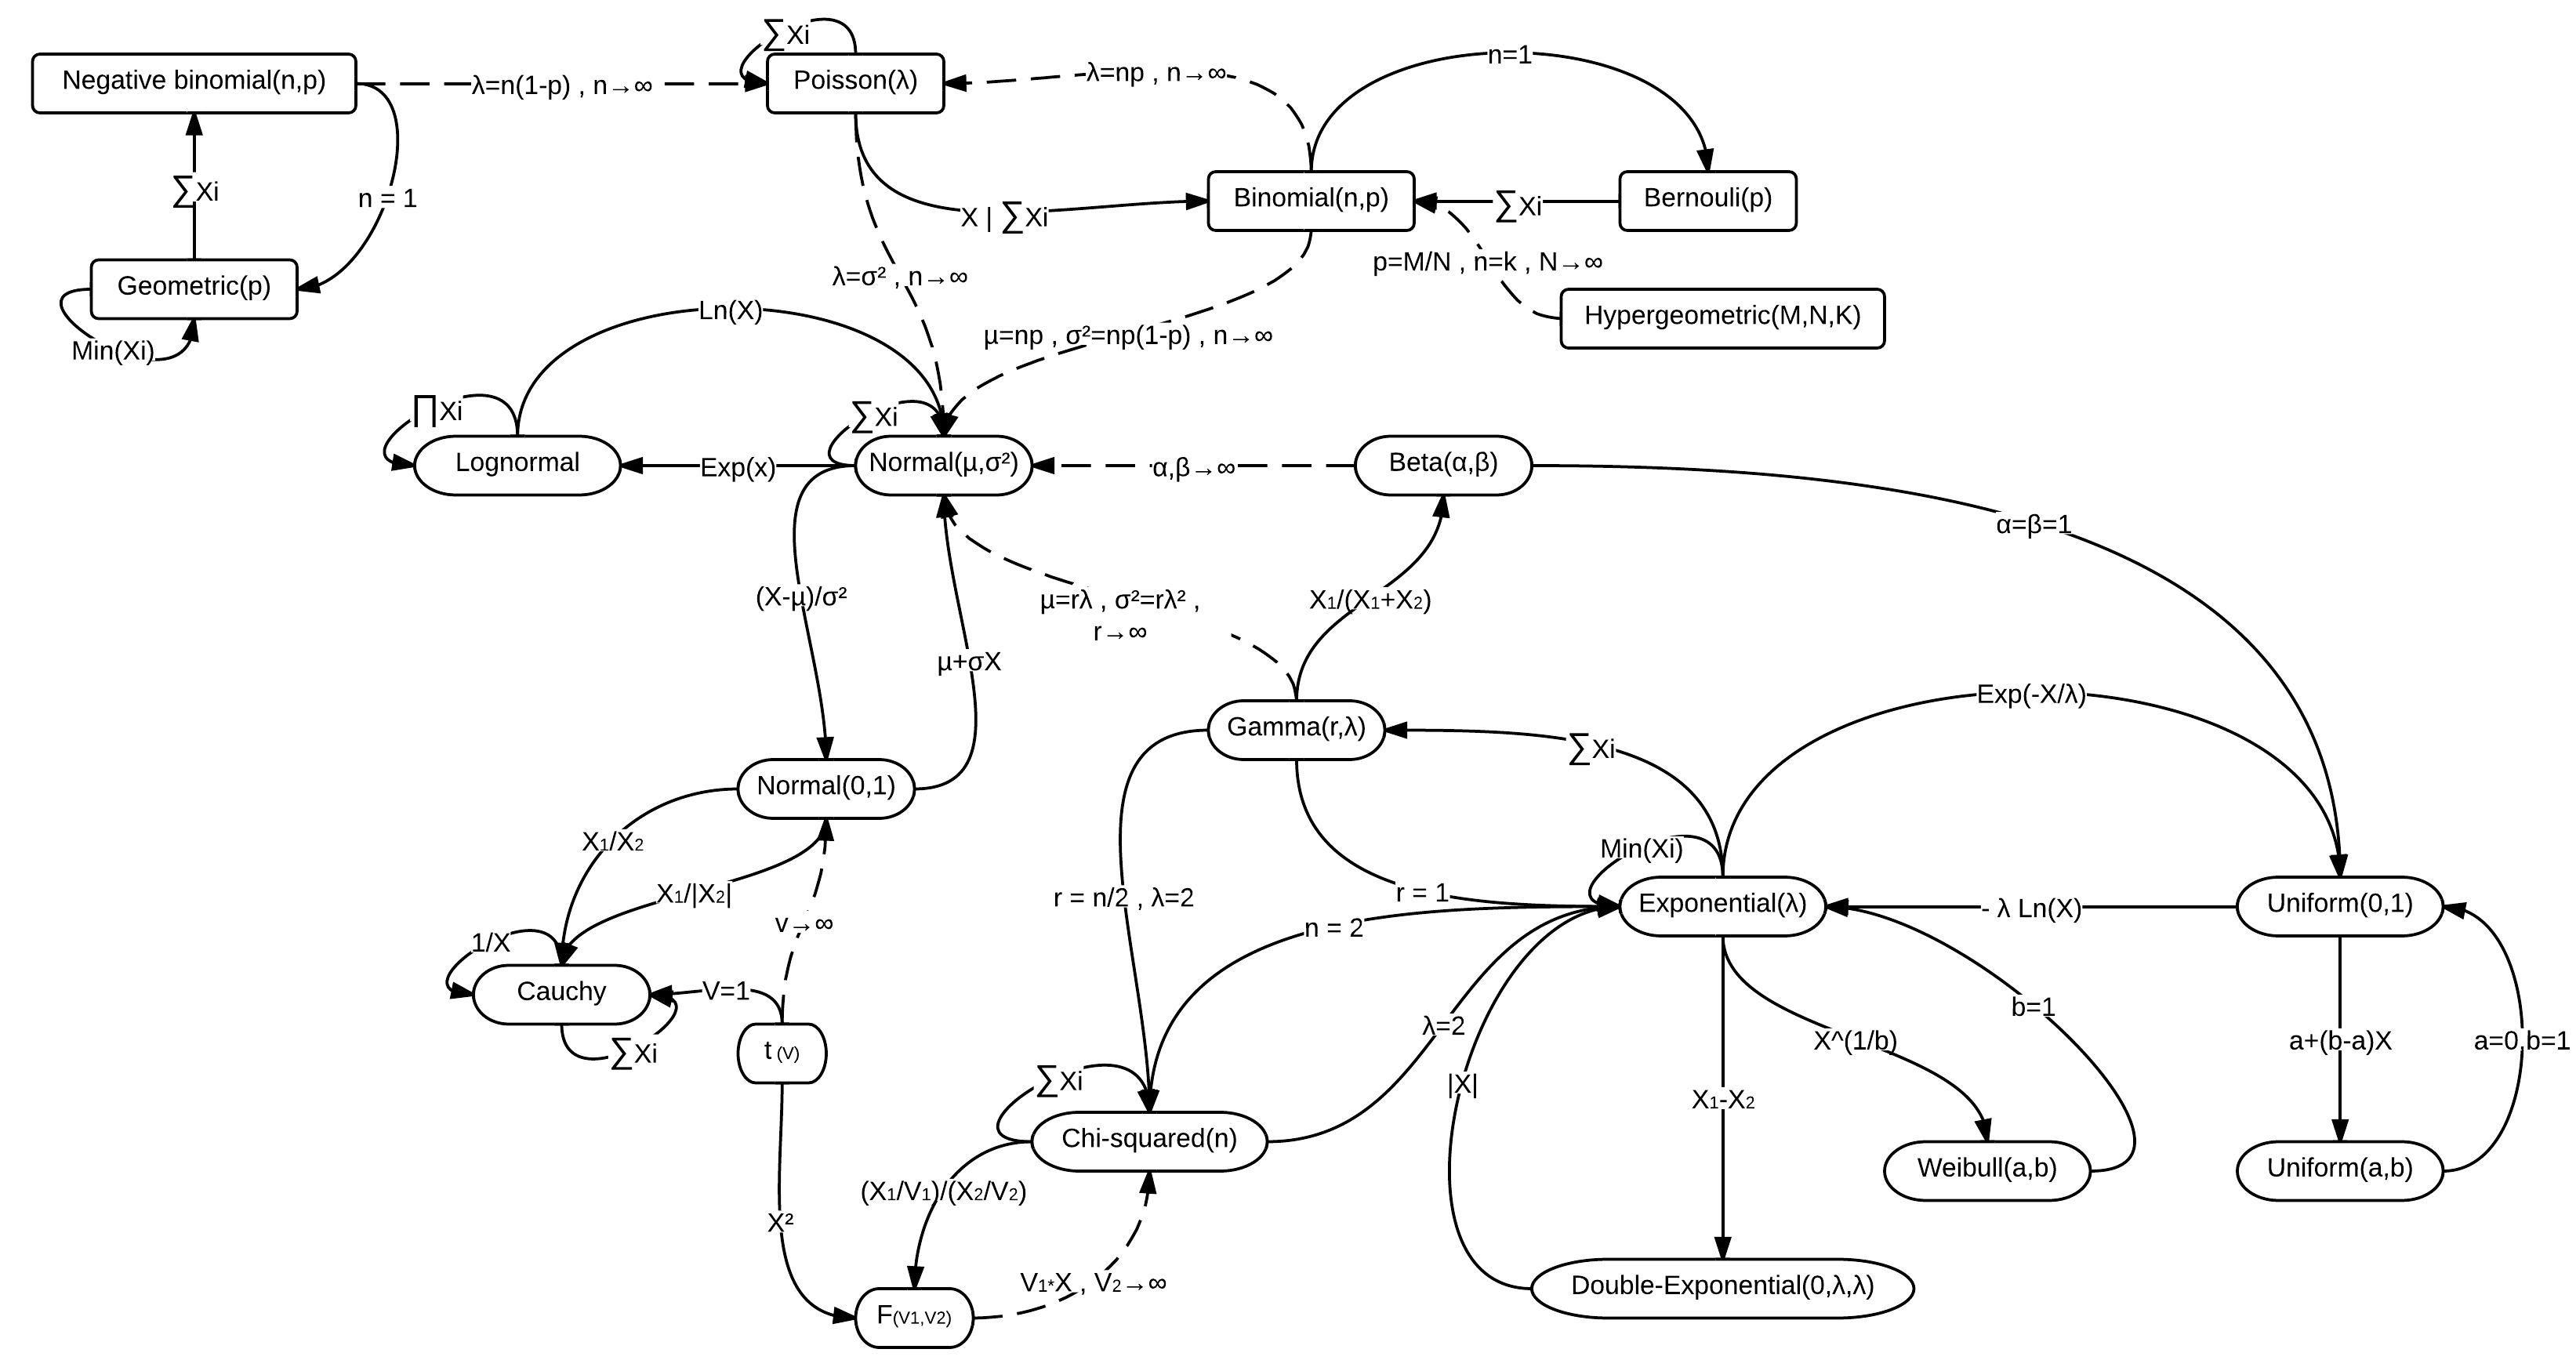
\includegraphics[scale=0.63]{Figures/RelacionesProbabilidad}
    \decoRule
    \caption[Relaciones entre algunas de las distribuciones de probabilidad univariadas]{Las relaciones entre algunas de las distribuciones de probabilidad univariadas se ilustran con líneas conectadas, las líneas discontinuas significan relación aproximada. [Fuente: \parencite{univariateDist}]}
    \label{fig:relacionesDistribuciones}
\end{figure}

\break

\section{Generación de distribuciones estadísticas para el simulador}

\subsection{Generación de variable aleatoria tipo \textit{Poisson}}
Como se revisó en la sección~\ref{generarGeoEstocastica}, uno de los requisitos para generar una geometría estocástica es que el número de puntos en el plano sea Poisson, es por esto que en esta sección se comprobó la generación de la variable aleatoria Poisson en Python usando la libreria \textit{scipy}.\newline

Para esto, se realizaron $10000$ generaciones de numeros siguiendo una distribución de Poisson con tasa $\lambda = 20$, se obtuvo el histograma de todos los números generados y se comparó con su función de masa de probabilidad (PMF).\newline

Se observa que la distribución del histograma sigue a la función masa de probabilidad de Poisson [\textit{véase Figura~\ref{fig:generacionPoisson}}], por lo que se valida la generación de números Poisson en Python.\newline

\begin{figure}[th]
    \centering
    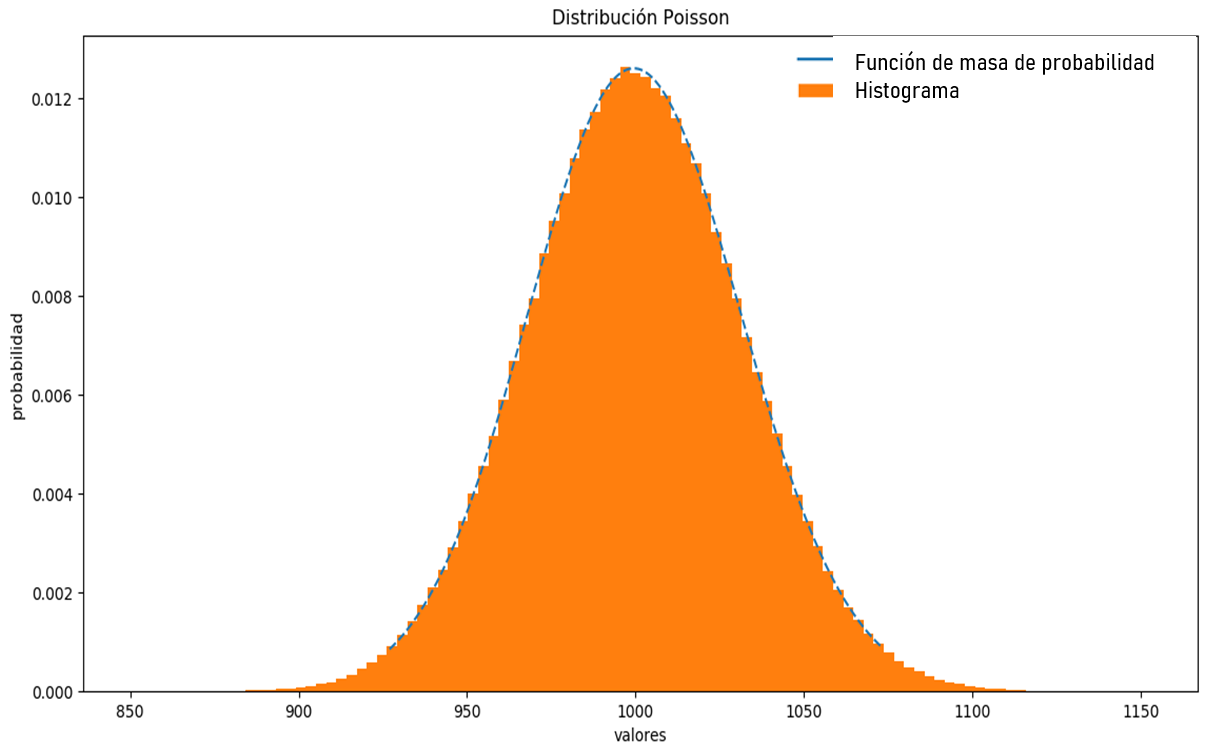
\includegraphics[scale=.5]{Figures/PoissonDistribution}
    \decoRule
    \caption[Gráfica comparación PMF e histograma de distribución Poisson en Python]{Gráfica comparación PMF e histograma de distribución Poisson en Python}
    \label{fig:generacionPoisson}
\end{figure}
\break

\subsection{Generación de variables aleatorias tipo \textit{Exponencial} y \textit{Rayleigh}}

Como se revisó en la sección~\ref{DesvRayleigC2}, cuando el desvanecimiento es de tipo Rayleigh, la magnitud o amplitud de la señal es Rayleigh y la potencia es exponencial. En esta sección, se comprobó la generación de estas variables aleatorias en Python usando la libreria \textit{random}.\newline

Se realizaron $10000$ generaciones de numeros siguiendo una distribución Exponencial negativa con media $\mu =1$, se obtuvo el histograma de todos los números generados y se comparó con su función de densidad de probabilidad (PDF).\newline

De la misma manera con la otra distribución, se realizaron $10000$ generaciones de numeros siguiendo una distribución Rayleigh con desviación estándar $\sigma = 1$, se obtuvo el histograma de todos los números generados y se comparó con su función de densidad de probabilidad (PDF).\newline

Se observa que la distribuciones de los histogramas siguen a su respectiva función densidad de probabilidad (PDF) [\textit{véanse Figuras~\ref{fig:generacionExpon} y \ref{fig:generacionRay} }], por lo que se valida la generación de números Exponenciales y Rayleigh en Python.\newline

\begin{figure}[th]
    \centering
    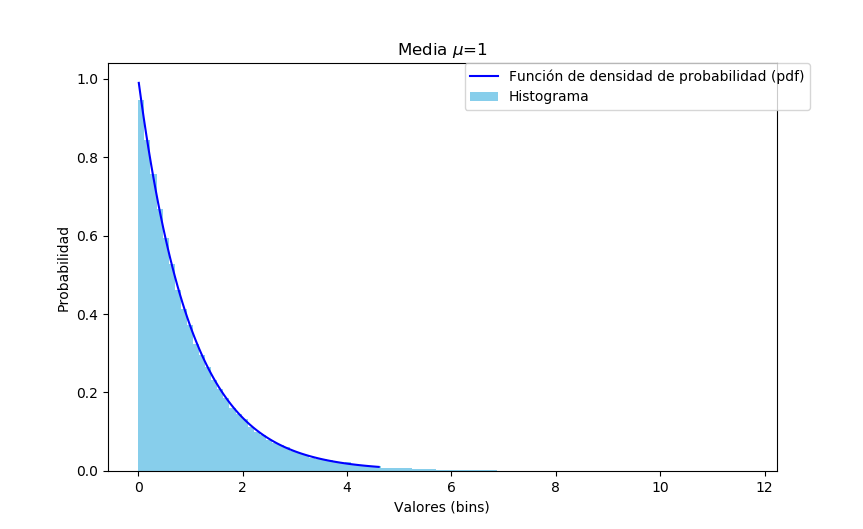
\includegraphics[scale=.6]{Figures/ExponentialDisitribution.png}
    \decoRule
    \caption[Gráfica comparación PDF e histograma de distribución Exponencial en Python]{Gráfica comparación PDF e histograma de distribución Exponencial en Python}
    \label{fig:generacionExpon}
\end{figure}

\begin{figure}[th]
    \centering
    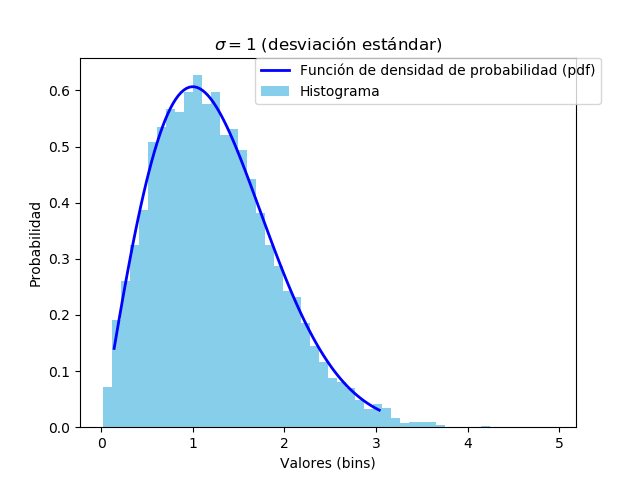
\includegraphics[scale=.7]{Figures/RayleighDistribution.png}
    \decoRule
    \caption[Gráfica comparación PDF e histograma de distribución Rayleigh en Python]{Gráfica comparación PDF e histograma de distribución Rayleigh en Python}
    \label{fig:generacionRay}
\end{figure}
\break

\subsection{Generación de variable aleatoria tipo \textit{Pareto}}

Como se revisó en la sección~\ref{Informesperiodicos}, la longitud de paquetes en la transmisión periodica siguió una distribución de Pareto con parámetro alfa = 2.5 y tamaño mínimo de carga útil de la aplicación = 20 bytes con un corte a 200 bytes.\newline

La distribución de Pareto a veces se conoce como el Principio de Pareto o la regla '80 –20 ', en este caso la regla establece que el 80\% de los tamaños de paquete que se formarán, los producirán solo el 20\% de los dispositivos del sistema y viceversa.\newline

La distribución de Pareto se puede replicar en Python usando el módulo Scipy.stats o NumPy. El módulo Scipy.stats abarca varias distribuciones de probabilidad y una biblioteca cada vez mayor de funciones estadísticas. Se comprobó la generación de esta variable aleatoria en Python usando la libreria \textit{scipy}.\newline

Se realizaron $100000$ generaciones de numeros siguiendo una distribución areto con parámetro alfa  $\alpha =2.5$ acotada entre 20 y 200, se obtuvo el histograma de todos los números generados y se comparó con su función de densidad de probabilidad (PDF).\newline

Se observa que la distribución del histograma sigue a la función densidad de probabilidad Pareto [\textit{véase Figura~\ref{fig:generacionPareto}}], por lo que se valida la generación de números Pareto en Python.\newline

\begin{figure}[th]
    \centering
    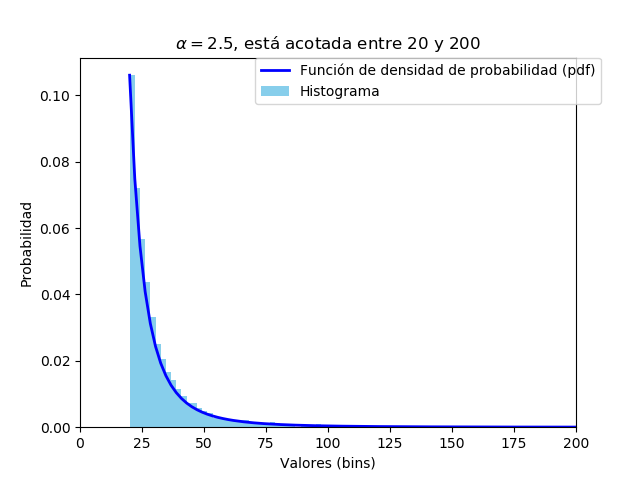
\includegraphics[scale=.7]{Figures/ParetoDIstribution}
    \decoRule
    \caption[Gráfica comparación PDF e histograma de distribución Pareto en Python]{Gráfica comparación PDF e histograma de distribución Pareto en Python}
    \label{fig:generacionPareto}
\end{figure}


%% Appendix B

\chapter{Simulación - Geometría celular hexagonal} % Main appendix title

\label{AppendixB} % For referencing this appendix elsewhere, use \ref{AppendixA}

\section{Generación de despliegue Uniforme de usuarios}

\section{Análisis de Geometría Celular un una celda}
%\include{Appendices/AppendixC}

%----------------------------------------------------------------------------------------
%	BIBLIOGRAPHY
%----------------------------------------------------------------------------------------

\printbibliography[heading=bibintoc]

%----------------------------------------------------------------------------------------

\end{document}  
